\section{Experiments}

In this section, we will briefly introduce the datasets and the compared methods. We will then further test the models' strength and generalizability with in-domain and cross-domain experiments, examine their efficacy and efficiency in early detection settings, and illustrate their explainability with examples. We will finally check the impact factors of risky post selection with controlled experiments.

\subsection{Datasets}

We adopt 3 datasets collected from Reddit in our experiment due to their public availability and wide acceptance in previous works \citep{losada2017erisk, trotzek2018utilizing,harrigian2020models}. They have different topic and label distribution, and also different content filtering strategy that aims to avoid label leakage and simulate user behaviors with different level of self-disclosure.

\paragraph{eRisk2017} consists of 137 depressed users and 755 control users and is divided into training/test set with 486/406 users each \citep{losada2016test}. The depressed users are identified with patterns like ``I was diagnosed with depression'', while the control users are those active on depression subreddit but had no depression. The posting year spans from 2007 to 2015. The anchor post for identification is filtered from the dataset.
% \KZ{since this is the same as one of the risky post templates, would it be consider info leak?}
% \ZL{Since depressed users can have different levels of self-disclosure, even if a direct revealing of diagnosis can be a realistic scenario, and Topic-Restricted actually can contain such information since it doesn't use the pattern matching. We consider 'info leak' as a consideration in dataset construction, and we just leave the datasets as they were, and won't tackle them in our work. But we do exhibit effectiveness across all these different settings.}

\paragraph{Topic-Restricted} consists of 6960 depressed users and 7683 control users, with a 8/1/1 random training/validation/test split \citep{wolohan2018detecting}. Since the original dataset is not released with the paper, we follow the implementation of \citet{harrigian2020models} to crawl the dataset ourselves in the same way. The depressed users are those who started a thread in depression subreddit while the control users are those who started a thread in AskReddit subreddit. The posting year spans from 2007 to 2021. For filtering, we removed all posts in mental health related subreddits.

\paragraph{RSDD} consists of 9210 depressed users and 107274 control users with a training/validation/test split of 39105/39122/39121, after data cleaning \citep{yates2017depression}. The depressed users are also identified with patterns, but further verified by annotators, while 12 control users are matched to a depressed user to minimize their distance of subreddit distribution. The posting year spans from 2006 to 2016. The filtering is the most strict among 3 datasets in that posts either posted in a mental health related subreddit or contain a depression-related term will be removed. 

\subsection{Competing Baseline Methods}
We compare our method with several competitive baselines. For traditional machine learning models. \textbf{LR} uses TF-IDF features and a logistic regression classifier. \textbf{Feature-Rich} utilizes some additional user-based features, including LDA topic distribution \citep{blei2003latent}, LIWC features \citep{pennebaker2001linguistic} and emoticon counts. This is a competitive baseline that has been widely accepted in depression detection works on Facebook, Twitter and Reddit datasets \citep{eichstaedt2018facebook,trotzek2018utilizing,harrigian2020models}

For neural baselines, due to their computational cost and length limit, post selection is necessary. Therefore, each method is denoted as a pair of model and selection strategy. For backbone model, we consider the strong pre-trained model \textbf{BERT} and the proposed \textbf{HAN-BERT}. For post selection strategy, \textbf{Heuristic} chooses last posts (eRisk2017, RSDD) or the first posts (Topic-Restricted)\footnote{The collection process of Topic-Restricted is temporally biased (find latest depression reddit first, and trace the history back), so that more depression related posts will appear at the end. We thus use the first posts to avoid the information leakage in time.} in user history. \textbf{Clus} and \textbf{Clus+Abs} are inspired by \citet{zogan2021depressionnet}. We use sentence-bert \citep{reimers-2019-sentence-bert} to get post embeddings and run K-means clustering to get the $K$ posts nearest to the cluster center as representative posts (Clus). These posts are further passed to a BART model \citep{lewis2020bart} pretrained on CNN/DM summarization dataset to get an abstractive summary (Clus+Abs). We also test the variants of our proposed screening strategy, including \textbf{Depress} using only 3 direct templates, \textbf{BDI-II} using 21 templates derived from BDI-II, and \textbf{Full} leveraging a combination of them. For RSDD, we additionally reproduce the \textbf{H-CNN} model \citep{yates2017depression}, which is a lightweight hierarchical CNN, and consume as many as 1,500 last posts.

For experiments on the eRisk2017 dataset, the basis of BERT and HAN-BERT models are \texttt{bert-base-uncased}. The sentence-bert model is \texttt{paraphrase-MiniLM-L6-v2}. The number of selected posts is $K=16$. We train with a batch size of 4, and learning rate of 2e-5. For experiments on the other datasets, we find that a tiny version of BERT\footnote{https://huggingface.co/prajjwal1/bert-tiny} is enough to achieve competitive results given the larger data size. We select 64 posts, and train with batch size = 32 and learning rate = 2e-4. We concatenate the selected posts as input into the BERT baselines. For HAN-BERT models, the user encoder is a 4-layer 8-head transformer encoder. To avoid the influence of randomness, we run each method with 3 different seeds and report the best performance.

\begin{table}[t]
    \centering
    \small
    \begin{tabular}{l|c}
        \hline
        {} & F1 \\
        \hline
        LR & 60.2 \\
        Feature-Rich & 63 \\
        \hline
        BERT (Clus) & 59.6 \\
        BERT (Clus+Abs) & 52.3 \\
        HAN-BERT (Heuristic) & 43.2 \\
        HAN-BERT (Clus) & 62.5 \\
        \hline
        HAN-BERT (Depress) & \textbf{70.5} \\
        HAN-BERT (BDI-II) & 66.0 \\
        HAN-BERT (Full) & 70.3 \\
        % - Attention & 67.9 \\
        \hline
    \end{tabular}
    \caption{\label{table:erisk2017} Results on eRisk2017 test set.}
\end{table}


\begin{table}[t]
    \centering
    \small
    \begin{tabular}{l|cc}
        \hline
        {} & Topic-Restricted & RSDD \\
        \hline
        LR & 69.8 & 52.1 \\
        Feature-Rich & 72.0 & 58 \\
        \hline
        H-CNN (last 1500) & - & 62.2 \\
        BERT (Clus) & 56.7 & - \\
        HAN-BERT$_{tiny}$ (Heuristic) & 68.0 & 38.2 \\
        HAN-BERT$_{tiny}$ (Clus) & 71.9 & - \\
        \hline
        HAN-BERT$_{tiny}$ (Depress) & 77.1 & \textbf{65.4} \\
        HAN-BERT$_{tiny}$ (BDI-II) & \textbf{78.9} & 60.1 \\
        HAN-BERT$_{tiny}$ (Full) & 77.1 & 61.1 \\
        \hline
    \end{tabular}
    \caption{\label{table:rsdd_wolohan} Test F1 on Topic-Restricted and RSDD dataset.}
\end{table}


\begin{table*}[th]
    \centering
	\small
    \begin{tabular}{l|cccccc}
        \hline
        Model & ERDE5 & ERDE50 & Precision & Recall & F1 & Time(s) \\
        \hline
        LR & 13.70 & 8.49 & 26.8 & 83.3 & 40.5 & 4710.7 \\
        Feature-Rich & 12.98 & 8.39 & 22.1 & \textbf{94.4} & 35.8 & 7558.4 \\
        HAN-BERT (Full) & \textbf{10.72} & \textbf{8.12} & \textbf{50.0} & 75.9 & \textbf{60.3} & \textbf{1330.3} \\
        \hline
    \end{tabular}
    \caption{\label{table:early} Test results on eRisk2017 in early detection setting. The lower ERDE5/50, the better model performs early detection.}
% \KZ{I'm wondering what if u include the results of HAN-BERT(BDI-II) here?
% Will it be an embarassment?}}
% \ZL{Their performance are similar, with one higher on some metrics and others good at other metrics. We thus chose a balanced and representative one for the simplicity of discussion.}
\end{table*}

\begin{table}[th]
    \centering
	\small
    \begin{tabular}{l|cc}
        \hline
        Source Domain & Topic-Restricted & RSDD \\
        \hline
        LR & 82.6 & 72.3 \\
        Feature-Rich & 85.7 & 75.3 \\
        \hline
        HAN-BERT$_{tiny}$ (Depress) & 86.6 & 82.9 \\
        HAN-BERT$_{tiny}$ (BDI-II) & \textbf{87.6} & 83.8 \\
        HAN-BERT$_{tiny}$ (Full) & 87.4 & \textbf{85.0} \\
        \hline
    \end{tabular}
    \caption{\label{table:cross} Test results (AUC) on eRisk2017 dataset with models trained on other domains.}
\end{table}

\subsection{In-Domain Results}
\label{sec:in-domain}

The in-domain test results are shown in Table \ref{table:erisk2017} and Table \ref{table:rsdd_wolohan}. On the eRisk2017 dataset (Table \ref{table:erisk2017}), we can see that BERT (Clus+Abs) performs worse than BERT (Clus), indicating that the abstractive summarization strategy does not necessarily work possibly due to the gap between its pretrained domain (News) and Reddit. HAN-BERT (Clus) outperforms BERT (Clus), showing the effectiveness of the proposed HAN structure. The poor performance of HAN-BERT (Heuristic) highlights the importance of post selection, and none of the traditional post selection methods can outperform the competitive Feature-Rich model with access to all posts. However, with our proposed screening strategy, the HAN-BERT models can significantly outperform baselines, suggesting the efficacy of these methods. Specifically, \textit{Depress} performs the best because this dataset don't enforce filtering of depression-related words so that strong direct depression signals remain in this dataset. \textit{BDI-II} and \textit{Full} also exhibit competitive performance by capturing indirect symptoms, and their performance can be further improved given more posts (\S \ref{sec:factor}). 

The results on the other 2 datasets are shown in Table \ref{table:rsdd_wolohan}. BERT (Clus) and HAN-BERT (Clus) don't show competitive performance on Topic-Restricted again, and requires expensive clustering stage, so we don't experiment them on the larger RSDD dataset. The proposed risky post screening based methods shows strong performance again, and are capable of outperforming both the traditional Feature-Rich (all posts) and another neural model H-CNN (1,500 posts) using only 64 posts and a tiny version of BERT. The orders between these screening methods differ across datasets possibly due to their differences in label distribution and filtering strategy, but their performances are overall competitive.

% \KZ{For in-domain results, the advantage of the BDI-II is not obvious,
% making the full not the best in all 3 cases. This is a bit disappointing.
% You need to explain, and do not use ``possibly because'', but give some
% concrete explainations. If possible do some more data analysis or
% look at intermediate results. Instead of F1, can we use AUC here as well?}
% \ZL{F1 is the standard, so we follow it. Full's AUC is actually slightly higher than Depress, but the overall advantage of HAN-BERTs' AUC over baselines are as big as F1.}

\subsection{Cross-Domain Results}

To test the cross-domain generalizability of different approaches, we train models on Topic-Restricted or RSDD first, and then test it directly on eRisk2017 test set. For HAN-BERT models on Topic-Restricted, we use the model trained with 64 selected posts, and also test on 64 posts selected with the same templates. For RSDD, we find that training and testing on 16 posts is enough to exhibit strong performance. In contrast to in-domain experiments using a fixed probability threshold 0.5 to decide the prediction, we don't apply this in cross-domain tests since the label distribution differs greatly between datasets, so that fixed threshold will lead to poor performance. Instead, we use a threshold-free metric, AUC, to measure the performance of each method.

The results are shown in Table \ref{table:cross}. Consistent with in-domain results, we find that Feature-Rich outperforms LR, and HAN-BERT models perform even better. The performance of LR and Feature-rich degrade significantly when trained on RSDD, since RSDD adopts a strict filtering strategy, excluding all posts in mental health related subreddits or containing a depression-related term, resulting in the huge differences between eRisk2017 and RSDD. Such domain gaps also cause the slight degradation of HAN-BERT (Depress), since it can access fewer direct depression expressions from the 2 source datasets than eRisk2017. On the other hand, HAN-BERT (BDI-II) and HAN-BERT (Full) generalize well, which indicates the usefulness of the theory-guided templates in selecting robust features across domains. Therefore, they can be especially useful in domains where people conceal their depression due to its stigmatization. The performance of all HAN-BERT models are more robust than baselines. This further suggests the generalizability of the proposed method.
% \KZ{If Full/BDI-II are not better than Depress in in-domain, but
% better than Depress in cross-domain, what does it mean? Need to explain
% carefully here.}

\begin{table*}[t]
    \centering
	\small
    \begin{tabular}{ccc}
        \hline
        Attention & Post & Diagnostic Basis \\
        \hline
        0.202 & \makecell[l]{It sucks that the Citalopram didn't work for you but glad to hear your other \\ meds are helping. It's my first time on antidepressants so I didn't know \\ what are their side effects.} & \makecell[c]{\textbf{Treatment} \\ Diagnosis \\ Changes in Appetite }\\
        \hline
        0.118 & \makecell[l]{Thanks! :) Sometimes it's really good to actually get the words out of  \\ me rather than internalising my feelings.} & \makecell[c]{Concentration Difficulty \\ Loss of Pleasure \\ \textbf{Self-Dislike}}\\
        \hline
        0.048 & \makecell[l]{Glad to know :) just glad I'm not working for the next couple of weeks. \\ Feel like I'm on a different planet haha.} & \makecell[c]{\textbf{Tiredness} \\ Stay still \\ Concentrate} \\
        \hline
        0.021 & \makecell[l]{Some films or TV shows. I remember watching ... The worst part was I'd  \\ already been laughed at by my mum for crying at the end of Breakfast at \\ Tiffanys (who leaves a cat out in the rain like that?). } & \makecell[c]{Sadness \\ \textbf{Crying} \\ Depressed Mood} \\
        \hline
        \end{tabular}
        \caption{\label{table:example} Example posting list (4 selected out of all 16 posts) of a user with depression with their attention weight in HAN and diagnostic basis according to top 3 cosine similarity (reasonable ones highlighted in bold).}
\end{table*}


\subsection{Early Detection}

We test model performance in the online early detection setting on eRisk2017 dataset, using the official metrics ERDE5 and ERDE50 \citep{losada2017erisk}. We also report Precision, Recall, F1 calculated using the early predictions (report positive if predicted probability over 0.5). To tackle the item-by-item updates, the baseline model LR and Feature-Rich will recalculate the features and run inference for each new post, while our HAN-BERT with risky post screening can deal this efficiently with the proposed evolving queue algorithm (\S \ref{sec:evolving}). When counting the running time, we accumulate the time costs for all posts no matter if the model makes early predictions to rule out the influence of early false positives. The baselines run on a Linux machine with CPU: E5-2678 (48 cores) and HAN-BERT runs with a NVIDIA 2080 Ti GPU. Although the comparison is not totally fair, we think it is still a practical setting for real world application.

The results are shown in Table \ref{table:early}. It can be seen that HAN-BERT (Full) significantly outperforms baselines in ERDE and F1, while also being faster. The reason for the superiority on effectiveness is because baselines produce much more false positives than HAN-BERT due to their sensitivity to single posts. The advantage of efficiency can be mainly attributed to the evolving queue algorithm, which greatly reduced the number of model inference to only 10.41\% of all posts. The efficient feature update also helps. Although the sentence encoding must be conducted for all posts, it only costs a small fraction of total time (114.7s out of 1330.3s). 
% \KZ{Do we have situations where the early detection result (e.g., using only 1/3 of the post sequences) of a user differs from the detection result of all the posts of the same user? That would be a flaw with the early detection framework? How do you explain that?}
% \ZL{Such case are actually common in practice, and that's why F1 of all methods drops significantly in Table 3 compares to Table 1. Since users may recover/suffer from depression at the middle, such changes are reasonable. And it can actually be a flaw in the current early detection framework. But we neither don't need, nor able to fix it in our work, since the actual period of depression cannot be known, even given the depression posts.}


\subsection{Lexical Analysis}

As has been shown in many previous works \citep{shen2017depression, eichstaedt2018facebook, wolohan2018detecting}, there are many significant lexical differences between the posts of depressed users and other users, which can be captured by the word frequency of certain categories in LIWC \citep{pennebaker2001linguistic}. For example, depressed users tend to use more \textbf{first person pronouns} (\textit{I}), words expressing \textbf{negative emotions} (e.g. \textit{hate, miss, alone}), and words about \textbf{health} (e.g. \textit{life, tired, sick}). Such lexical discrepancies do not only exist between the two groups of users, but also within the posts of depressed users themselves. Since our post screening method is expected to select the most risky posts, we hypothesize that the selected posts will exhibit more lexical depression indicators than other posts of depressed users. Therefore, we take the posts of depressed users in the eRisk2017 test set, and count the frequency of words in the 3 LIWC categories stated above. We then compare the proportion of these words in selected posts and other posts, and test their differences with two-sided proportion $z$ test.

\begin{figure}[h]
    \centering
    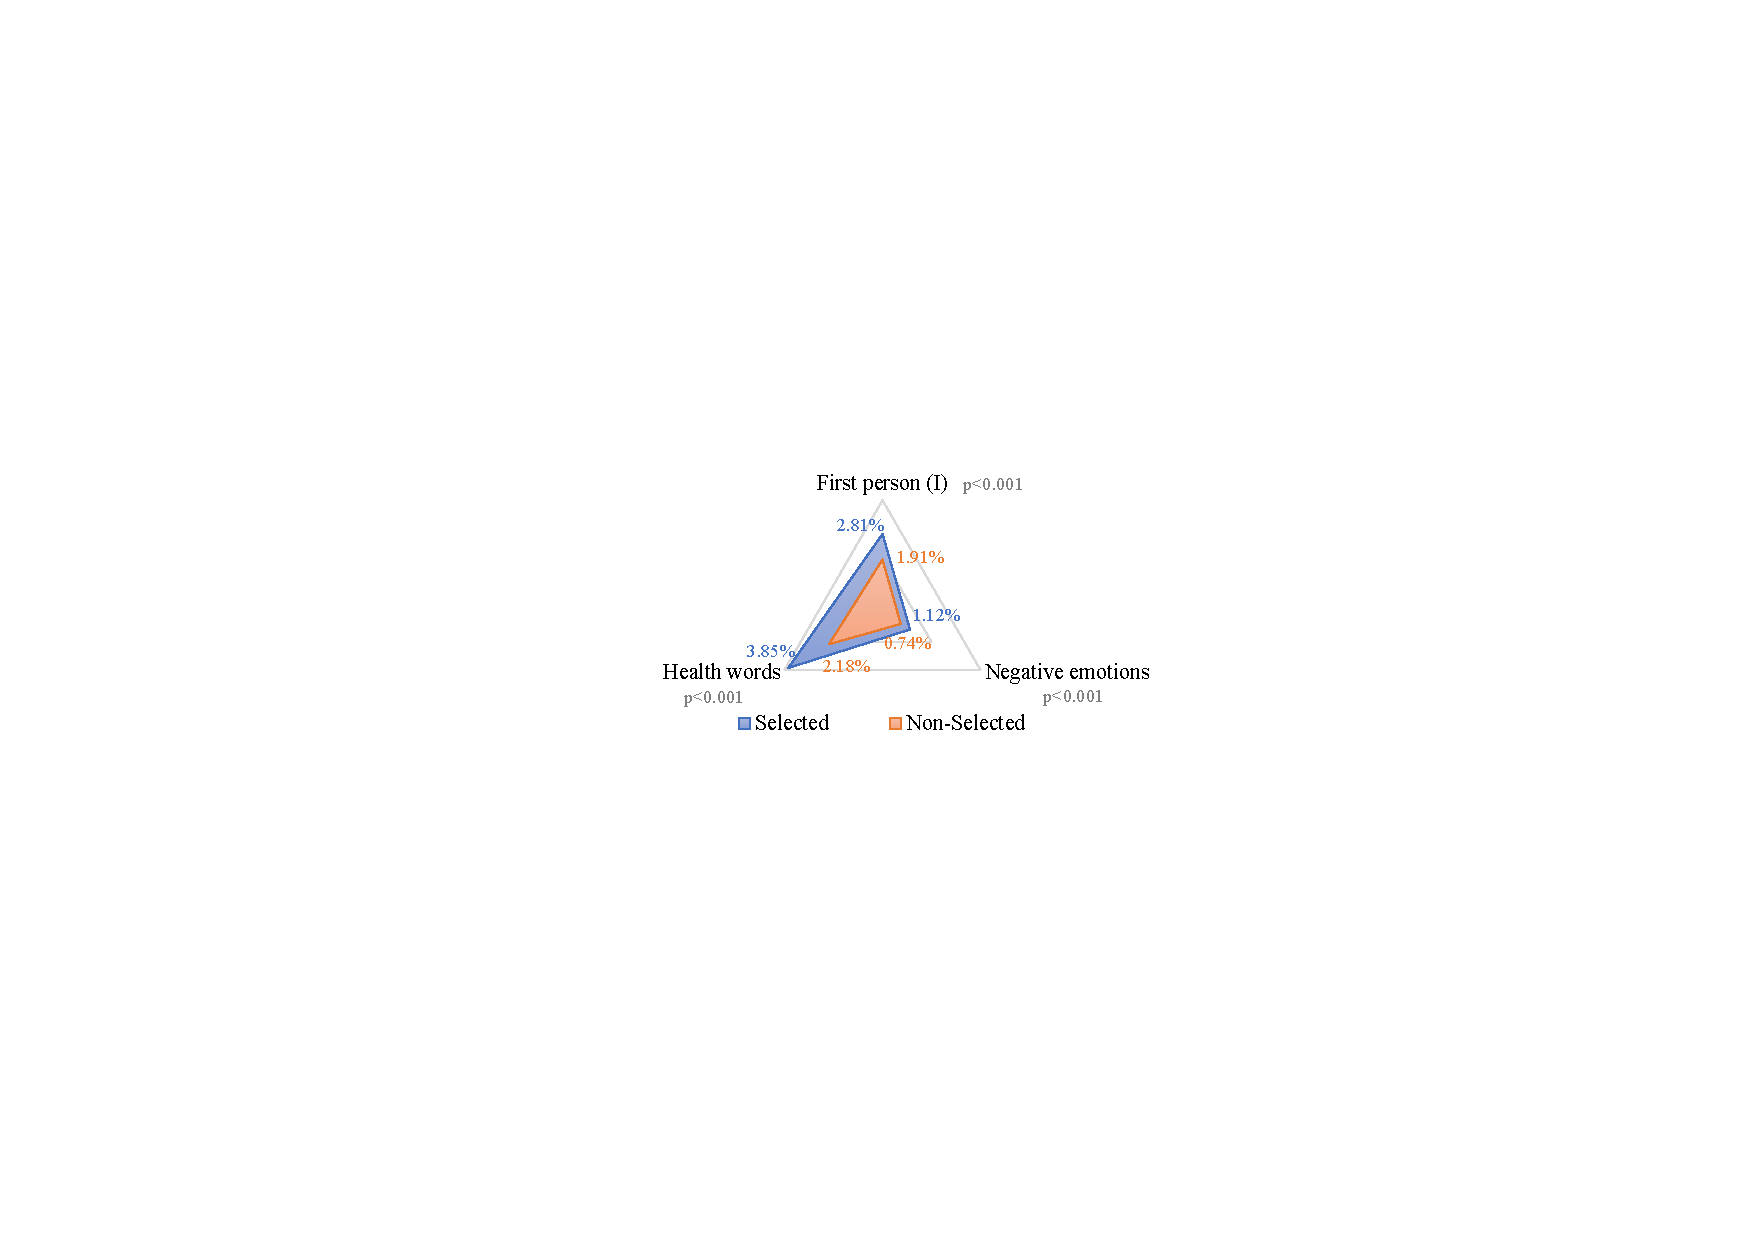
\includegraphics[width=0.9\columnwidth]{figures/lexical.pdf}
    \caption{Difference between selected and non-selected posts w.r.t. proportion of words in typical depress related LIWC categories.}
    \label{fig:lexical}
\end{figure}

As is illustrated in Figure \ref{fig:lexical}, there are also significant differences between the use of first person words, negative emotions and health-related words in selected (risky) and non-selected posts ($p < 0.001$ for all categories). The difference between risky posts and other posts of depressed users (Negative Emotion: 1.12\% vs. 0.74\%) can be even bigger than the difference between non-risky posts of depressed users and all posts from non-depressed users (Negative Emotion: 0.74\% vs. 0.79\%). This suggests that the proposed Risky Post Screening can still preserve strong lexical depression indicators, and can further eliminate normal posts that can mislead the model prediction.

\subsection{Qualitative Example}

We provide a concrete example in Table \ref{table:example} to analyze the behaviors of the proposed method in detail. From the column of attention weight, we can see that posts with strong depression indicators (e.g. antidepressants, internalizing feelings, see Row 1, 2) received much higher attention than a uniform baseline (1/16 = 0.0625), while posts with no evident signals of depression or even with a positive emotion (Row 3, 4) received low attention. This suggests the usefulness of the attention weight as an explanation for model prediction. The diagnostic bases decided by the cosine similarity between post and depression templates constitute another type of intuitive explanation. The top 3 diagnostic bases can usually capture the typical depression behaviors that the post may indicate, which can act as a convincing interpretation in its clinical applications. However, we noticed that sometimes the similarity model may rank an unreasonable aspect high in the list of bases, such as the ``Sadness'' for the last positive post. We owe such mistakes to the limitation of sentence representation models, such as not sensitive to negation \citep{ribeiro2020beyond}. We expect that stronger sentence representation models may lead to further improvement.

We also exhibit that our method has the potential to track the fluctuations in depressive mood for depression patients by another example (Figure \ref{fig:curve}). We produce such curve with the following procedure. First, we group posts according to a 14-day interval. Then we use HAN-BERT (Full) to conduct post screening and depression detection to get a predicted probability for each post group. To produce a smooth curve along time, we design a moving average strategy to derive a more stable depression score from predicted depression probabilities. Suppose the predicted probability of group $i$ is $pr_i$, and the depression score is $s_i$. Then we have 
$$s_1 = pr_1, s_i = \alpha s_{i-1} + (1-\alpha) pr_{i-1} (i > 1)$$
where 
$$\alpha = max(0, 0.5 * \frac{28-t_{\Delta}}{28-1})$$
$t_{\Delta}$ is the time interval between the first post of two groups measured in days. Therefore, if two groups are close in time, then the score from the last period will have a higher influence on the next score. Finally, we plot the curve according to the moving-averaged scores.

As we can see in Figure \ref{fig:curve}. In addition to the accurate detection of depression, the proposed method may also be able to capture the changes in the severity of depression symptoms. The model reported a high risk when the user expressed typical depression symptoms like frustrations (A) or worthlessness (C), and also reported low depression score when the user actually showed interest in things (B), which might indicate a recovery from the symptom of ``Loss of Interest''. The overall trend is in line with the user's self-report that the depression comes cyclically like waves.

\subsection{Impact Factors of Risky Post Screening}
\label{sec:factor}

Here we study the impact of 2 design choices of risky post screening.

\paragraph{Number of Posts} 
We study the effect of post numbers on the Topic-Restricted dataset (Figure \ref{fig:post_numbers}). It can be seen that all methods can get further improvement given more posts, and scale-based methods can benefit more possibly because more posts can help cover more diverse expressions of depression symptoms, which cannot be fully captured given a small size limit.


\begin{figure}[h]
    \centering
    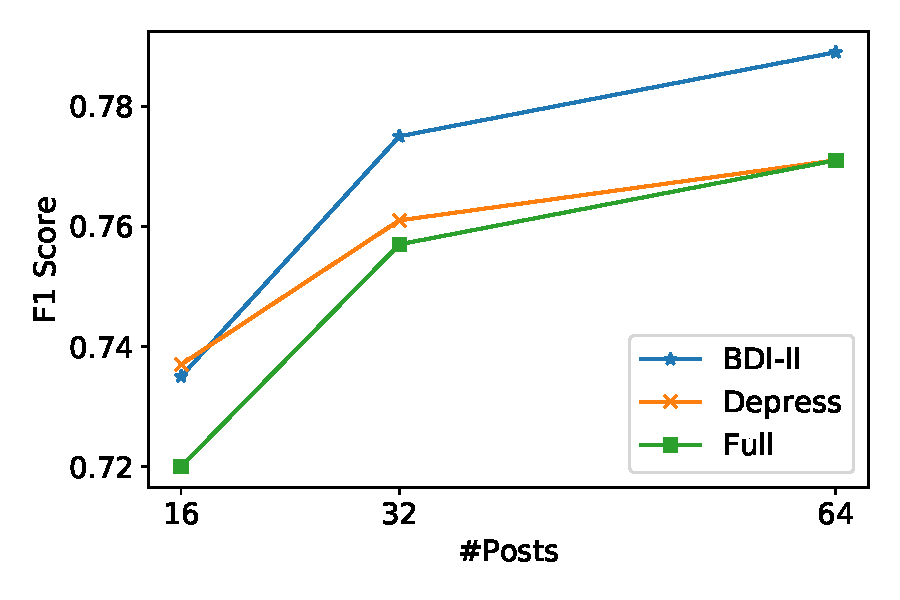
\includegraphics[width=0.88\columnwidth]{figures/post_numbers.pdf}
    \caption{Effect of number of posts on Topic-Restricted.}
    \label{fig:post_numbers}
\end{figure}

\begin{table}[th]
    \centering
	\small
    \begin{tabular}{l|c}
        \hline
        Depression Scale & F1 \\
        \hline
        BDI-II & \textbf{70.3} \\
        HDRS & 68.0 \\
        CES-D & 67.9 \\
        PHQ-9 & 67.2\\
        \hline
        HDRS+BDI-II+PHQ-9 & \textbf{72.1} \\
        HDRS+BDI-II+CES-D & 70.5 \\
        \hline
    \end{tabular}
    \caption{\label{table:different scales} Test results on eRisk2017 dataset with different depression scales and their combinations.}
\end{table}

\begin{figure*}[th]
    \centering
    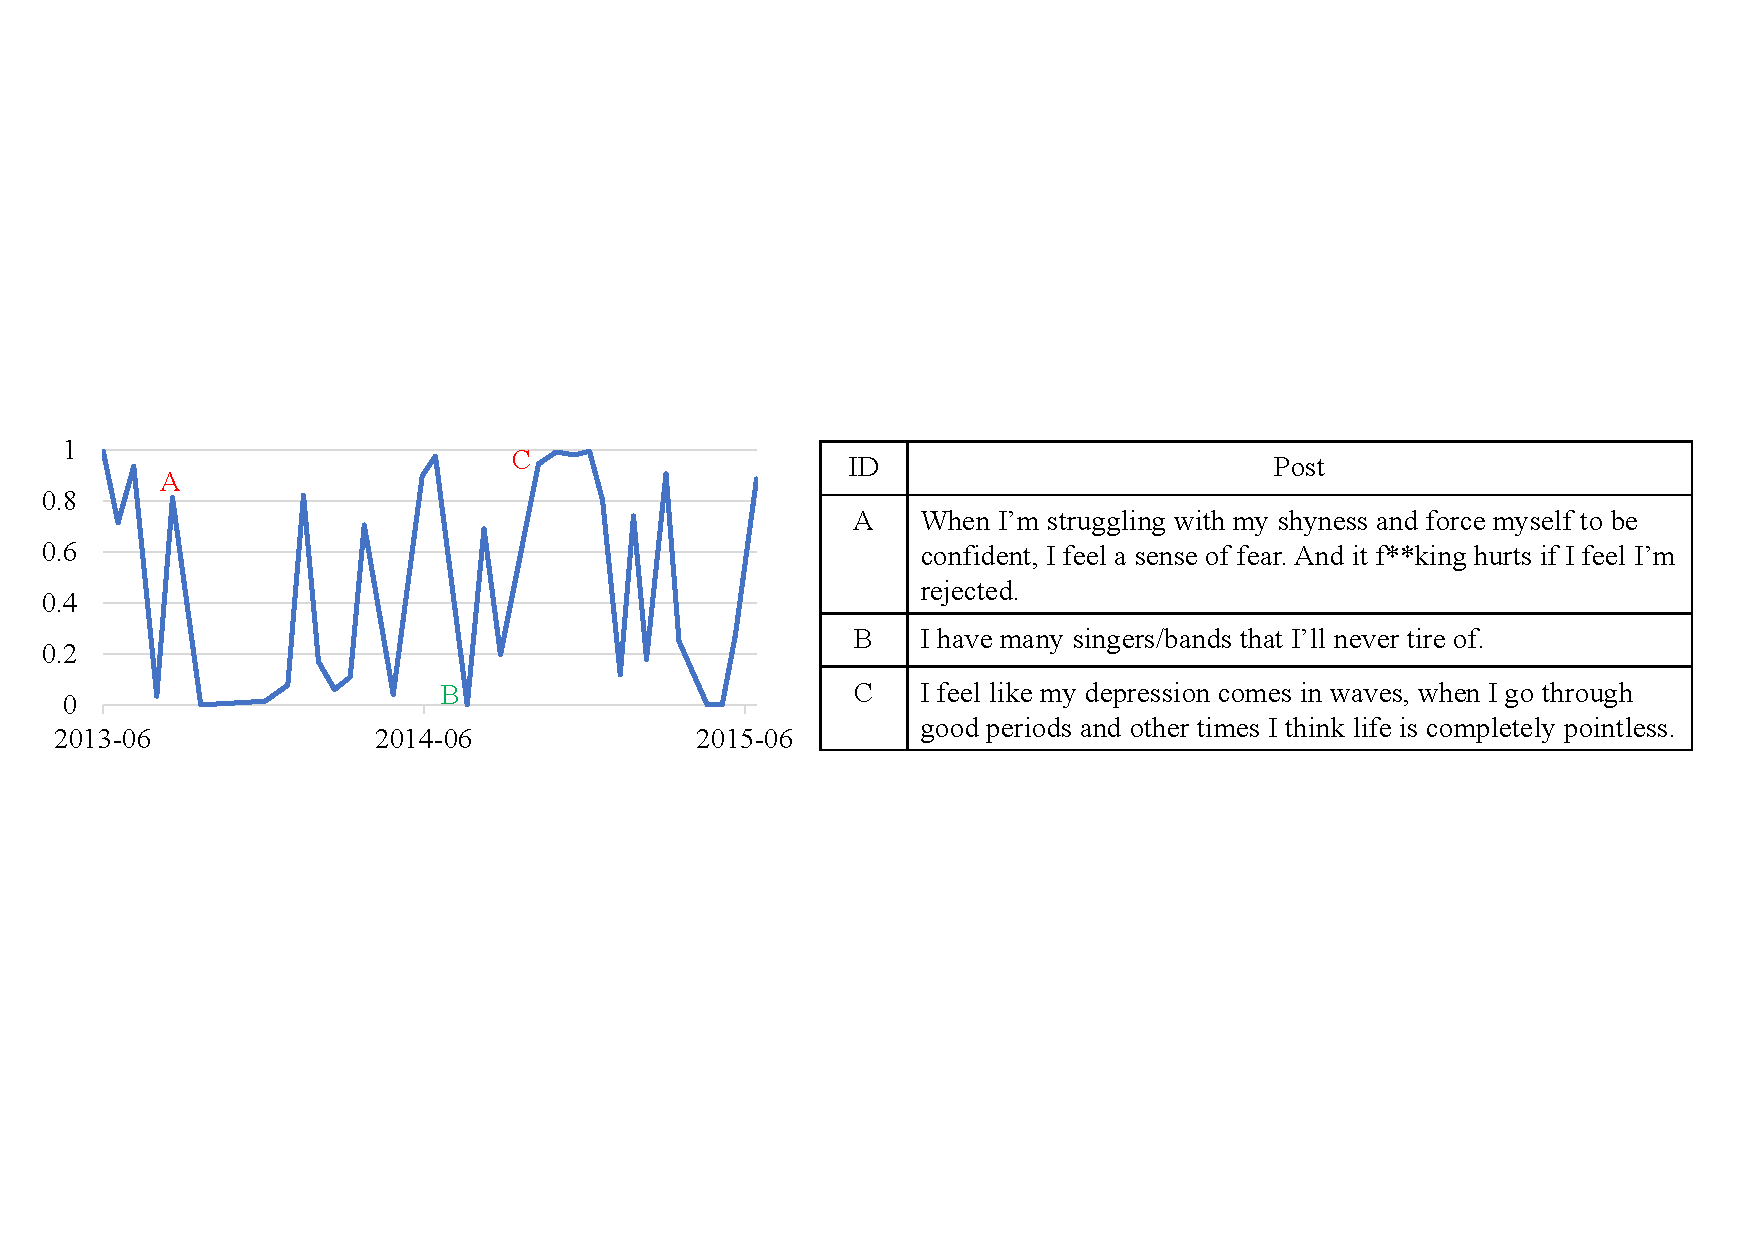
\includegraphics[width=2\columnwidth]{figures/curve.pdf}
    \caption{Predicted depression score by HAN-BERT (Full) along with time for a user in eRisk2017 dataset. We selected 3 time periods on predicted peaks and troughs, and show a representative post in each period.}
    \label{fig:curve}
\end{figure*}

\paragraph{Different Scales}
We explore three other commonly-adopted scales besides BDI-II, including HDRS \citep{hamilton1986hamilton}, CES-D \citep{Lenore1977CES-D} and PHQ-9 \citep{kroenke2001phq}, with similar approaches to rewrite the dimensions into depression templates. We also tried Majority Voting of models paired with different scales. Their performance on eRisk2017 dataset in shown in Table \ref{table:different scales}. We found that BDI-II is the single best performing scale. The combination of HDRS, BDI-II and PHQ-9 reaches the highest performance for their highly complementary dimensions. 

